
\documentclass[]{report}
\voffset=-1.5cm
\oddsidemargin=0.0cm
\textwidth = 480pt


\usepackage{amsmath}
\usepackage{graphicx}
\usepackage{amssymb}
\usepackage{framed}
\usepackage{multicol}
%\usepackage[paperwidth=21cm, paperheight=29.8cm]{geometry}
%\usepackage[angle=0,scale=1,color=black,hshift=-0.4cm,vshift=15cm]{background}
%\usepackage{multirow}
\usepackage{enumerate}

\usepackage{amsmath,amsfonts,amssymb}
\usepackage{color}
\usepackage{multirow}
\usepackage{eurosym}
\usepackage{framed}

%\input def.tex
%\input dsdef.tex
%\input rgb.tex

%\newcommand \la{\lambda}
%\newcommand \al{a}
%\newcommand \be{b}
\newcommand \x{\overline{x}}
\newcommand \y{\overline{y}}

\begin{document}
	
3.10 Correlated Equilibria
Consider the following battle of the sexes game
C F
C (2,5) (0,0)
F (0,0) (5,2)
1 / 39

%=======================================================================%
\subsection{3.10 Correlated Equilibria}
\begin{itemize}
\item Up to now it has been assumed that the players choose their
strategies independently of each other, i.e. there is no
communication.
\item However, in coordination (and anti-coordination games) it would
help players to communicate in order to choose an equilibrium
which is ”favourable to both”.
\item For example, in the game above the players could agree to toss a
coin and if the result is heads, then both play C. Otherwise, both
play F.
\item This would be an ”equitable” solution to the game. Both players
would receive an expected reward of 3.5.
\end{itemize}
%%- 2 / 39

%=======================================================================%
%%- Correlated Equilibria
\begin{itemize}
\item One important feature of the solution presented above is that given
the result of the coin toss, neither player wishes to depart from the
agreed action given that the other player keeps to the agreement.
\item For example, given the result is heads, the proposed action pair is
(C, C). If player 1 changes unilaterally from this action, then she
obtains 0 rather than 2.
\item This is the essence of a correlated equilibrium: given the signal
available to each player (here, they jointly observe the result of a
coin toss), none of them can gain by ignoring the signal given the
others take the appropriate action.
\item In general, we assume that each player receives his/her own private
signal. In certain cases (discussed later), we may assume that the
signal is public (observed by all the players).
\end{itemize}

%%- 3 / 39

%=======================================================================%
\subsection{Definition of a Correlated Strategy Pair in a 2-Player Game}
A correlated strategy pair is given by a joint distribution over the
set of pure strategy pairs. For example, the correlated strategy
described for the battle of the sexes game is
C F
C
1
2
0
F 0
1
2
i.e. with probability 0.5 (after a heads) both play C, otherwise
both play F.
4 / 39

%=======================================================================%
\subsection{Definition of a Correlated Strategy Pair in a 2-Player Game}
It should be noted that given the action to be taken by one player
under such a correlated strategy pair, the action to be taken be the
other is known. In such cases, the strategy pair can be achieved by
the players jointly observing a public signal.
Otherwise, it is assumed that players each observe a private signal
telling them which action to take. The joint distribution of the
signals corresponds to the joint distribution of the actions to be
taken.
5 / 39

%=======================================================================%
\subsection{Relations Between Correlated Strategy Pairs, Pure and
Mixed Strategies}
Suppose both players have two possible actions. The general form
of a correlated strategy pair is
C D
A p1 p2
B p3 p4
, where p1 + p2 + p3 + p4 = 1. Such a correlated strategy can be
presented as a 4-dimensional vector π = (p1, p2, p3, p4).
6 / 39

%=======================================================================%
\subsection{Expected Rewards Under a Correlated Strategy Pair}
This correlated strategy pair means that (A, C) is played with
probability p1, (A, D) is played with probability p2, etc.
The expected reward of Player i under correlated strategy π is
denoted Ri(π) and calculated with respect to the joint distribution
of the actions to be taken, i.e. the payoff of Player i is given by
Ri(π) = p1Ri(A, C) + p2Ri(A, D) + p3Ri(B, C) + p4Ri(B, D).
This is a linear combination of the pi
.
%% 7 / 39

%=======================================================================%
\subsection{Relations Between Correlated Strategy Pairs, Pure and
Mixed Strategies}
\begin{itemize}
	\item If pi = 1 for some i, then the correlated strategy pair is a pair of
	pure strategies.
	\item 	For example, π = (0, 1, 0, 0) corresponds to the pair of pure
	strategies (A, D).
	\item 	If π is of the form (qr, q[1 − r], [1 − q]r, [1 − q][1 − r]), then it
	corresponds to a pair of mixed strategies.
	\item 	In this case, Player 1 takes action A with probability q and Player
	2 takes action C with probability r (independently of the action of
	Player 2).
\end{itemize}

%% 8 / 39

%=======================================================================%
\section{Relations Between Correlated Strategy Pairs, Pure and
Mixed Strategies}
It follows that the set of correlated strategy pairs is an extension of
the set of mixed strategy pairs.
In general, communication is required to attain a correlated
strategy pair.
It is assumed that the form of a correlated strategy pair and the
way in which it is to be achieved is agreed upon before the game is
played.
However, it is assumed that this agreement is not binding (and
cannot be made binding). Hence, players are free to ignore the
action recommended to them.
9 / 39

%=======================================================================%
\subsection{Conditions for a Correlated Equilibrium in a 2×2 Matrix
Game}
According to the correlated strategy pair
C D
A p1 p2
B p3 p4
Player 1 is advised (by the appropriate signalling procedure) to play
A with probability p1 + p2. Given Player 1 is advised to play A, the
probability that Player 2 is advised to play C is p1
p1+p2
.
10 / 39

%=======================================================================%
%%- \subsection{Conditions for a Correlated Equilibrium in a 2×2 Matrix Game}
\begin{itemize}
	\item 
\end{itemize}
Each player should maximise their expected reward given the signal
(recommendation) he/she receives.
Hence, if Player 1 obtains the recommendation to play A, her
expected reward under such a correlated strategy pair is
p1R1(A, C)
p1 + p2
+
p2R1(A, D)
p1 + p2
.
If she ignores this recommendation (from the linearity of her
expected payoff, we may assume that she plays B), her expected
reward is
p1R1(B, C)
p1 + p2
+
p2R1(B, D)
p1 + p2
.
11 / 39

%=======================================================================%
\subsection{Conditions for a Correlated Equilibrium in a 2×2 Matrix
Game}
For stability, we require that
\[p1R1(A, C)
p1 + p2
+
p2R1(A, D)
p1 + p2
≥
p1R1(B, C)
p1 + p2
+
p2R1(B, D)
p1 + p2
.\]
This leads to
\[p1R1(A, C) + p2R1(A, D) ≥ p1R1(B, C) + p2R1(B, D).\]
12 / 39

%=======================================================================%
\subsection{Conditions for a Correlated Equilibrium in a 2×2 Matrix
Game}
It should be noted that if p1 = p2 = 0, then the above derivation
does not make sense (since we divide by 0).
However, in this case Player 1 is never recommended to play A and
so we may ignore this condition.
However, in this case the final inequality is simply 0 ≥ 0, which is
satisfied (i.e. in practice this condition is ignored when
p1 = p2 = 0).
13 / 39

%=======================================================================%
%% Conditions for a Correlated Equilibrium in a 2×2 Matrix Game
Arguing in a similar way, the 4 conditions for a correlated
equilibrium are
p1R1(A, C) + p2R1(A, D)≥p1R1(B, C) + p2R1(B, D)
p3R1(B, C) + p4R1(B, D)≥p3R1(A, C) + p4R1(A, D)
p1R2(A, C) + p3R2(B, C)≥p1R2(A, D) + p3R2(B, D)
p2R3(A, D) + p4R2(B, D)≥p2R2(A, C) + p4R2(B, C)
These conditions correspond in turn to the following
recommendations: 1) Player 1 to play A, 2) Player 1 to play B, 3)
Player 2 to play C and 4) Player 2 to play D.
14 / 39

%=======================================================================%
%=======================================================================%
\subsection{Relation Between Nash Equilibria and Correlated Equilibria}
\begin{itemize}
	\item Any Nash equilibrium pair of strategies is also a Correlated
	Equilibrium. A pair of mixed strategies that is not a Nash
	equilibrium is not a correlated equilibrium.
	\item	Any randomisation over Nash equilibria is also a correlated
	equilibrium. 
		\item Any randomisation over a set of strong Nash equilibria
	can be attained by joint observation of a public signal.
	\item	For example, in the battle of the sexes game, both (F, F) and
	(C, C) are strong Nash equilibrium. 
	\item Any correlated strategy pair
	that picks (F, F) with probability p and otherwise picks (C, C) is a
	correlated equilibrium.
\end{itemize}

%%- 15 / 39

%=======================================================================%
Relation Between Nash Equilibria and Correlated Equilibria
There is also a mixed Nash equilibrium where Player 1 plays C
with probability 2
7
and Player 2 plays C with probability 5
7
.
Presented as a correlated equilibrium, this corresponds to
C F
C
2
7 ×
5
7 =
10
49
2
7 ×
2
7 =
4
49
F
5
7 ×
5
7 =
25
49
5
7 ×
2
7 =
10
49
16 / 39

%=======================================================================%

\subsection{Choosing a Correlated Equilibrium}
\begin{itemize}
	\item Since any Nash equilibrium is a correlated equilibrium and multiple
	Nash equilibria may occur, it is clear that there may well be
	multiple correlated equilibria.
	\item	Hence, if the problem of the choice of a Nash equilibrium exists,
	then the problem of the choice of a correlated equilibrium also
	exists.
	\item	However, the concept of correlated equilibrium assumes that
	communication is possible and hence players may choose an
	appropriate equilibrium based on some criterion.
		\item First we consider
	the set of attainable payoffs.
\end{itemize}

%%- 17 / 39
\subsection{The Set of Attainable Payoffs Under a Correlated Strategy
Pair}
Consider the following game (an example of the chicken game).
F C
F (0,0) (8,2)
C (2,8) (6,6)
18 / 39

%=======================================================================%
%%- The Set of Attainable Payoffs Under a Correlated Strategy Pair
\begin{itemize}
\item For example, by randomising between the Nash equilibria (C, F)
and (F, C), any vector of expected payoffs on the line between
(8, 2) and (2, 8) can be attained.
\item  Similarly, we can attain a vector of expected payoffs anywhere on
any of the lines between the payoff vectors given by any two pairs
of strategies.
\item  By randomising between 3 or more strategy pairs, we can obtain
any payoff vector within the interior of the lines obtained above.
\item  It follows that the set of attainable payoffs is the convex hull of the
payoff vectors given in the payoff matrix (the smallest convex set
that contains all these vectors).
\end{itemize}
%%- 19 / 39

\subsection{The Set of Attainable Payoffs Under a Correlated Strategy
Pair}
\begin{itemize}
	\item This set can be obtained by joining the points given by each payoff
	vector in the payoff matrix.
	\item 	The external set of lines thus drawn is the boundary of the convex
	hull (set of attainable payoffs).
	\item 	The convex hull for the chicken game considered above is
	illustrated on the following slide.
\end{itemize}

20 / 39
%=======================================================================%
\subsection{The Set of Attainable Payoffs Under a Correlated Strategy
	Pair}

\begin{figure}
\centering
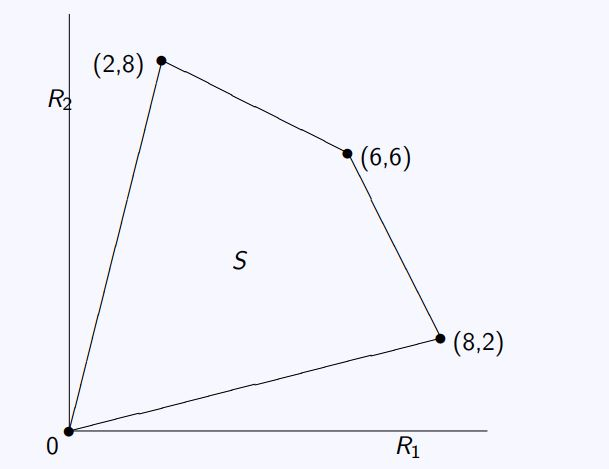
\includegraphics[width=0.7\linewidth]{images/DR9-Slide47}
\caption{}
\label{fig:DR9-Slide47}
\end{figure}
%- 21 / 39
%=======================================================================%

%=======================================================================%
%\subsection{The Set of Attainable Payoffs Under a Correlated Strategy Pair}
\begin{itemize}
	\item Note that the maximum payoff attainable by a player must occur
	at one of the vertices of the convex hull (i.e. be attained when a
	pair of pure strategies is played).
\item	Similarly, the sum of the payoffs must be maximised for some pair
	of pure strategies.
\end{itemize}

22 / 39
%=======================================================================%
\subsection{The Set of Pareto Optimal Payoff Vectors}
\begin{itemize}
	\item A payoff vector is Pareto optimal if it is a) attainable and b) there
	is no attainable payoff vector for which one player attains a greater
	payoff and the other player obtains at least the same payoff.
	\item For the chicken game, it can be seen that the set of Pareto optimal
	solutions is the union of the line from (2,8) to (6,6) and the line
	from (6,6) to (8,2).
	\item This is the top right border of the set of
	attainable payoffs.
\end{itemize}

%% 23 / 39

%=======================================================================%
\subsection{Choosing a Correlated Equilibrium}
\begin{itemize}
	\item For example, the solution presented for the battle of the sexes
	game equalises the payoff of the players while maximising the sum
	of the expected payoffs (the sum of the payoffs cannot be more
	than 7).
	\item	An equilibrium which maximises the sum of the expected payoffs of
	the players is called a utilitarian equilibrium.
	\item An equilibrium which maximises the expected payoff of Player i is
	called a Libertarian i equilibrium.
	\item	An equilibrium which maximises the minimum expected payoff of a
	player is called an egalitarian equilibrium. From the argument
	given above, the coin tossing solution is an egalitarian equilibrium.

\end{itemize}
%-	24 / 39

%=======================================================================%
\subsection{Deriving an Appropriate Correlated Equilibrium}
\begin{itemize}
	\item Since the expected payoffs of the players are linear combinations of
	the pi (probabilities of choosing the particular strategy pairs), the
	criteria given above involve maximising a linear combination of pi
	.
	\item The conditions for a correlated equilibrium are given by a set of
	linear inequalities involving the pi
	.
	\item Equilibria of the types given above can be derived by defining the
	problem as a linear programming problem.
	\item In many cases we can derive appropriate correlated equilibria using
	mathematical argumentation, rather than using the more general
	simplex method.
\end{itemize}

%% -25 / 39
%=======================================================================%
\subsection{Deriving an Appropriate Correlated Equilibrium}
Consider the battle of the sexes game
C F
C (2,5) (0,0)
F (0,0) (5,2)
26 / 39

%=======================================================================%
%% \subsection{Deriving an Appropriate Correlated Equilibrium}
The linear programming problem defining the Libertarian 1
equilibrium is given by
max z = 2p1 + 0p2 + 0p3 + 5p4 = 2p1 + 5p4
subject to
1) the conditions for (p1, p2, p3, p4) to define a joint distribution,
i.e. pi ≥ 0, i = 1, 2, 3, 4 and p1 + p2 + p3 + p4 = 1,
2) the conditions for (p1, p2, p3, p4) to be a correlated equilibrium
(see next slide).
27 / 39

%=======================================================================%
%%- Deriving an Appropriate Correlated Equilibrium
The conditions for a correlated equilibrium are
2p1 + 0p2 ≥ 0p1 + 5p2⇒p1 ≥
5p2
2
0p3 + 5p4 ≥ 2p3 + 0p4⇒p4 ≥
2p3
5
5p1 + 0p3 ≥ 0p1 + 2p3⇒p1 ≥
2p3
5
0p2 + 2p4 ≥ 5p2 + 0p4⇒p4 ≥
5p2
2
%%- 28 / 39

%=======================================================================%
%%- Deriving an Appropriate Correlated Equilibrium
\begin{itemize}
	\item We could find the appropriate solution by solving this linear
	programming problem. But such problems are often easy to solve if
	we first derive the Nash equilibria.
	\item	The pure Nash equilibria are (C, C) and (F, F). The strategy pair
	(F, F) gives the maximum possible payoff to Player 1 (over the set
	of pure stratergy pairs) and is a Nash equilibrium (and thus a
	correlated equilibrium).
	\item	Hence, (F, F) must be the correlated equilibrium which maximises
	the payoff of Player 1.
	\item	Similarly, (C, C) is the correlated equilibrium which maximises the
	payoff of Player 2.
\end{itemize}

%%- 29 / 39

%=======================================================================%
%%- Deriving an Appropriate Correlated Equilibrium
Now consider the utilitarian equilibrium. The problem in this case
is
\[max z = (2 + 5)p1 + (0 + 0)p2 + (0 + 0)p3 + (5 + 2)p4 = 7p1 + 7p4,\]
subject to the same conditions as before.
Again, knowing the pure Nash equilibria for this problem, we can
calculate the (set of) utilitarian equilibria.
(F, F) and (C, C) are Nash equilibria which maximise the sum of
the payoffs to the players (over the set of pure strategy pairs).
30 / 39

%=======================================================================%
%%- Deriving an Appropriate Correlated Equilibrium
Any randomisation over these two Nash equilibria is a correlated
equilibrium and gives the same sum of payoffs.
Hence, any π of the form π = (p, 0, 0, 1 − p) is a utilitarian
equilibrium.
31 / 39

%=======================================================================%
%% \subsection{Deriving an Appropriate Correlated Equilibrium}
\begin{itemize}
	\item Now consider the egalitarian equilibrium. This battle of the sexes
	is not symmetric, but there is a degree of symmetry in the payoffs
	that implies that at an egalitarian equilibrium both players have
	the same expected payoff.
	\item	A 2×2 matrix game where both players can choose either action A
	or action B will be called ”quasi-symmetric” if
	R1(i, j)=R2(j, i),
	R1(i, i)=R2(j, j), where i 6= j, i, j ∈ {A, B}.
	i.e. a payoff vector on the leading diagonal is the reverse of the
	other payoff vector on that diagonal.
		\item Note that a symmetric game
	is quasi-symmetric.
\end{itemize}

%%- 32 / 39

%=======================================================================%
%=======================================================================%
%% \subsection{Deriving an Appropriate Correlated Equilibrium}
\begin{itemize}
	\item Result At an egalitarian equilibrium of a quasi-symmetric game,
	both players must obtain the same expected payoff.
\item It follows that to find an egalitarian equilibrium of a
	quasi-symmetric game, one should maximise the expected sum of
	the payoffs subject to a) the standard constraints for a correlated
	equilibrium (stability and the conditions required for a distribution)
	and b) the constraint that both players should obtain the same
	payoff.
\end{itemize}

33 / 39

%=======================================================================%
%=======================================================================%
\subsection{Deriving an Appropriate Correlated Equilibrium}
In this case the problem (as before) is to maximise z = 7p1 + 7p4,
but with the additional constraint that the payoffs of the players
are equal, i.e.
2p1 + 5p4 = 5p1 + 2p4 ⇒ p1 = p4.
Any correlated equilibrium of the form (p, 0, 0, 1 − p) maximises
the sum of the expected payoffs.
Setting p =
1
2
, the player’s expected payoffs are equalised and
hence the egalitarian equilibrium is ( 1
2
, 0, 0,
1
2
).
34 / 39
%=======================================================================%
\subsection{Graphical Presentation/Interpretation of the Solution}
The set of attainable payoffs is given by
R2
R1
•
•
•
✦✦✦✦✦✦✦✦✦✦
☞
☞
☞
☞
☞
☞
☞
☞
☞
☞❅❅
❅
❅
❅
❅
0
(5,2)
(2,5)
S
35 / 39

%=======================================================================%
%=======================================================================%
\subsection{Graphical Presentation/Interpretation of the Solution}
There are 2 pure Nash equilibria which give payoff vectors of (2, 5)
and (5, 2), respectively.
The set of Pareto optimal solutions is the line between these two
payoff vectors, i.e. any Pareto optimal solution can be obtained by
appropriately randomising between the two Nash equilibria.
Thus any Pareto optimal solution can be obtained at a correlated
equilibrium.
In such a case the solution of the equilibrium choice problem can
be solved by choosing the appropriate payoff vector from the set of
Pareto optimal payoff vectors and defining the corresponding
randomisation over the pure Nash equilibria.
36 / 39

%=======================================================================%
%=======================================================================%
%%- \subsection{Graphical Presentation/Interpretation of the Solution}
Hence, the Libertarian 1 equilibrium has to attain a payoff vector
of (5, 2) (the Pareto optimal payoff which maximisses the payoff of
Player 1). The corresponding correlated strategy is (F, F) (in
terms of a strategy pair) or (0, 0, 0, 1) (in terms of the standard
description of a correlated strategy).
Similarly, the Libertarian 2 equilibrium is (C, C) [or (1, 0, 0, 0)] and
gives a payoff of (2, 5).
37 / 39

%=======================================================================%
%=======================================================================%
%%- \subsection{Graphical Presentation/Interpretation of the Solution}
In this battle of the sexes game, each Pareto optimal solution gives
the same sum of payoffs. Thus, any mixture between (C, C) and
(F, F) is a utilitarian equilibrium.
The payoff at the egalitarian equilibrium is given by the element of
the set of Pareto optimal payoffs at which the minimum payoff to
either of the players is maximised.
This condition is achieved if either a) both players obtain the same
expected payoff, or b) if one player always gets more than the
other at a Pareto optimal payoff vector, then we maximise the
payoff of the player with the minimum reward.
In this case, we should equalise the payoffs of the players. It
follows that both players should obtain 7
2
and the appropriate
correlated equilibrium is to choose (F, F) with probability 0.5,
otherwise choose (C, C).
%%- 38 / 39

%=======================================================================%
\subsection{Graphical Presentation/Interpretation of the Solution}
\begin{itemize}
	\item Hence, the derivation of appropriate correlated equilibria is
	relatively straightforward when any Pareto optimal payoff vector
	can be attained at a correlated equilibrium.
	\item	It should be noted that in the Chicken game (C, C) is not a Nash
	equilibrium (and is hence not a correlated equilibrium), but the
	corresponding payoff vector, (6, 6), is an element of the set of
	Pareto optimal payoff vectors.
	\item	It follows that not all Pareto optimal payoff vectors can be attained
	by a correlated equilibrium and the choice of an appropriate
	correlated equilibrium may be more difficult.
	\item	This problem will be considered in the tutorials.
\end{itemize}

%%- 39 / 39


\end{document}